\section{Case Study: Library Management System}

\subsection{Introduction}

Online Library Management System is a system which
maintains the information about the books present in the
library, their authors, the members of library to whom
books are issued, library staff and all.

This is very difficult to organize manually.
Maintenance of all this information
manually is a very complex task.
Owing to the advancement of technology, organization of an Online Library becomes much simple.

The Online Library Management has been designed to computerize and
automate the operations performed over the information
about the members, book issues and returns and all other
operations. This computerization of library helps in many
instances of its maintenances. It reduces the workload of
management as most of the manual work done is reduced.

\subsection{Objective}

The main objective of this project is to develop a system that
will help in maintaining the information about the books present in the library, their authors, the members of library to whom books are issued, library staff and all.

The library management system keeps track of reader with the following considerations:

\begin{enumerate}
    \item The system keeps track of the staff with a single point
          authentication system comprising login ID and password.
    \item Staff maintains the book catalog with its ISBN, Book title, price(in INR), category(novel, general, story), edition, author
          Number and details.
    \item A publisher has publisher ID, Year when the book was
          published, and name of the book.
    \item Readers are registered with their user ID, email,
          name (first name, last name), Phone no (multiple entries allowed), communication address. The staff keeps track of readers.

    \item Readers can return/reserve books that stamps with issue
          date and return date. If not returned within the prescribed time period, it may have a due date too.
    \item Staff also generate reports that have readers ID, registration number of report, book number and return/issue info.
\end{enumerate}

\subsection{Design}

The following are the entities of the system:

\subsubsection{Entities}

\begin{itemize}
    \item \textbf{Book}

          It has authno, isbn number, title, edition, category,
          price. ISBN is the Primary Key for Book Entity.
    \item \textbf{Reader}

          It has UserId, Email, address, phone no, name.
          Name is composite attribute of firstname and lastname. Phone No. is multivalued attribute. UserId is the Primary Key for Readers
          entity.
    \item \textbf{Publisher}

          It has PublisherID, Year of publication,
          name. PublisherID is the Primary Key.
    \item \textbf{Authentication System}

          It has LoginID and password
          with LoginID as Primary Key.
    \item \textbf{Reports}

          It has UserId, Reg\_no, Book\_no, Issue/Return
          date. Reg\_no is the Primary Key of reports entity.
    \item \textbf{Staff}

          It has name and staff\_id with staff\_id as Primary Key.
    \item \textbf{Reserve/Return Relationship Set}

          It has three attributes:
          Reserve date, Due date, Return date.
\end{itemize}

The relationships between the entities are as follows:

\subsubsection{Relationships}

\begin{itemize}
    \item A reader can reserve N books, but one book can be reserved by
          only one reader. The relationship 1:N.
    \item A publisher can publish many books, but a book is published by
          only one publisher. The relationship 1:N.
    \item Staff keeps track of readers. The relationship is M:N.
    \item Staff maintains multiple reports. The relationship 1:N.
    \item Staff maintains multiple Books. The relationship 1:N.
    \item Authentication system provides login to multiple staffs. The relation is 1:N.

\end{itemize}

\pagebreak

\subsubsection{ER Diagram}

\begin{figure}[ht]
    \centering
    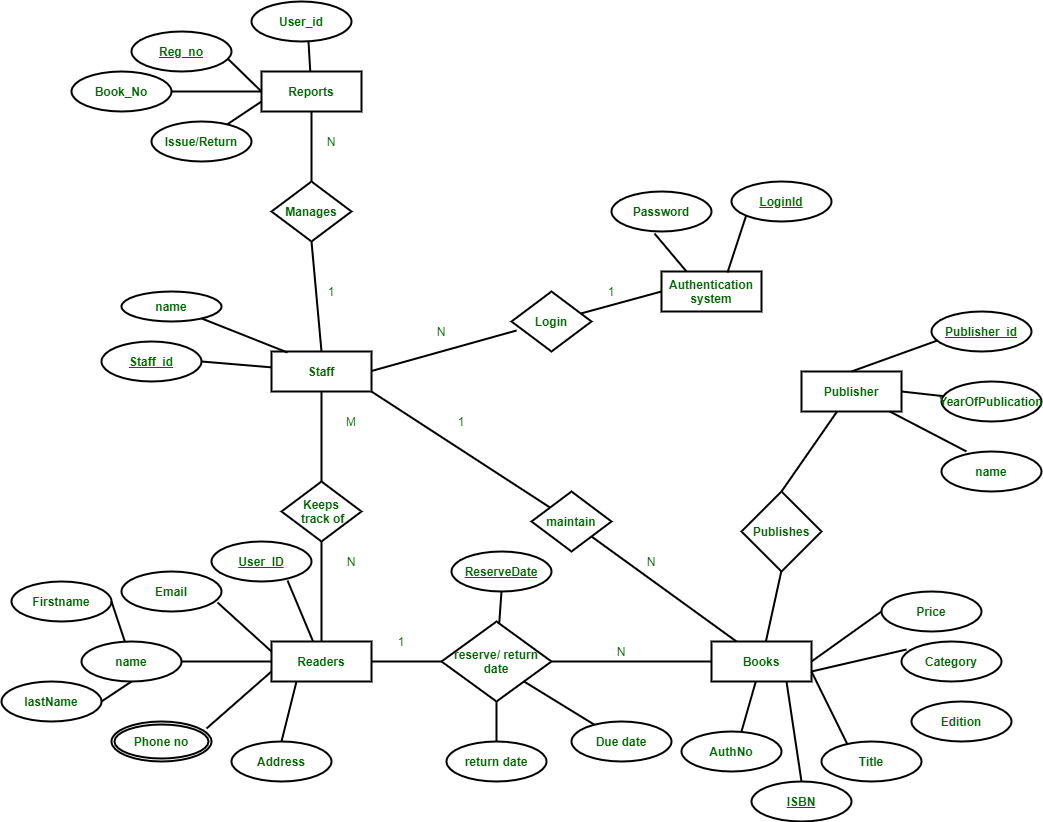
\includegraphics[width=0.9\textwidth]{res/libraryER.png}
    \caption{ER Diagram}
    \label{fig:er-diagram}
\end{figure}
